\documentclass{article}

\usepackage[palatino]{mypackages}\usepackage{mycommands}

\usepackage{verbatim}
\usepackage[active,tightpage]{preview}
\PreviewEnvironment{tikzpicture}
\setlength\PreviewBorder{5pt}

\begin{document}


\begin{tikzpicture}[rounded corners]

  \node at (6,18) {\Huge{Genau einer der Briefe ist mit einigen seiner Kreise verbunden.}};

  \node at (0,0) {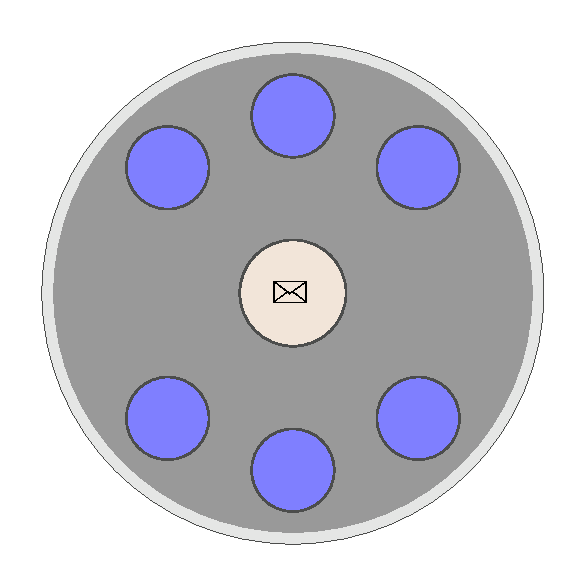
\includegraphics{105_pdfsam_Brief-Kreise-Blau.pdf}};

  \node at (12,0) {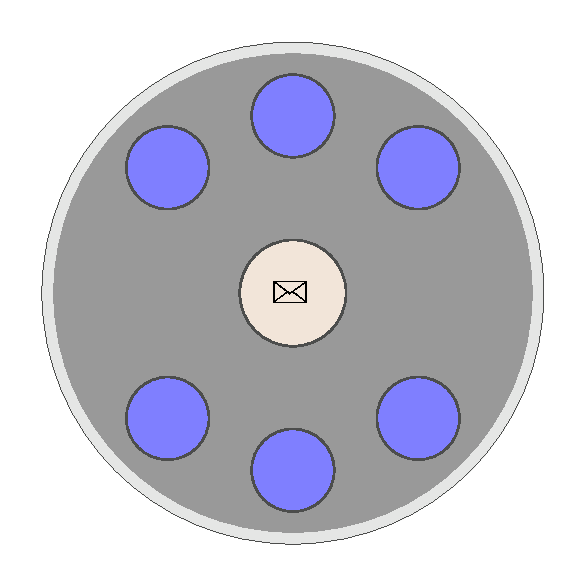
\includegraphics{105_pdfsam_Brief-Kreise-Blau.pdf}};

  \node at (12,12) {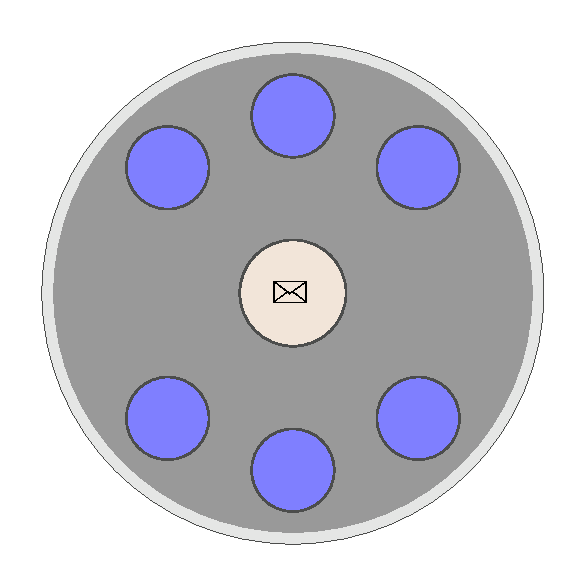
\includegraphics{105_pdfsam_Brief-Kreise-Blau.pdf}};

  \node at (0,12) {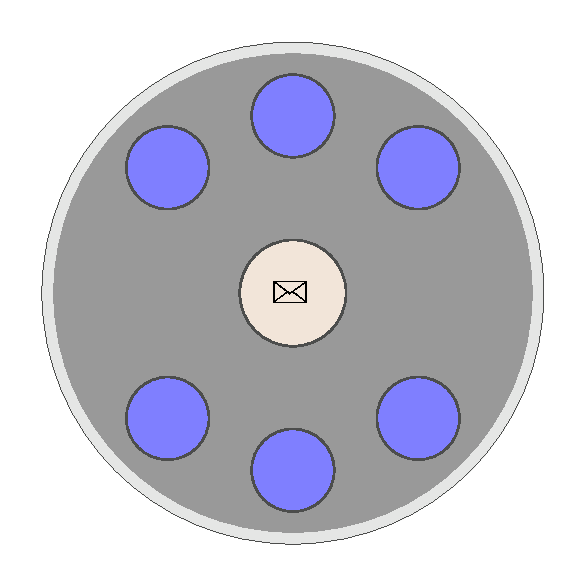
\includegraphics{105_pdfsam_Brief-Kreise-Blau.pdf}};

  \node[draw=black!80,fill=blue!30,ultra thick] at (0,-6)
  {\Huge{Wahr}};

  \node[draw=black!80,fill=blue!30,ultra thick] at (6,-6)
  {\Huge{Falsch}};

  \node[draw=black!80,fill=blue!30,ultra thick] at (12,-6) {\Huge{Mehr Info}};


\end{tikzpicture}

\begin{tikzpicture}[rounded corners]

  \node at (6,18) {\Huge{Genau einer der Briefe ist mit einigen seiner Kreise verbunden.}};

  \node at (0,0) {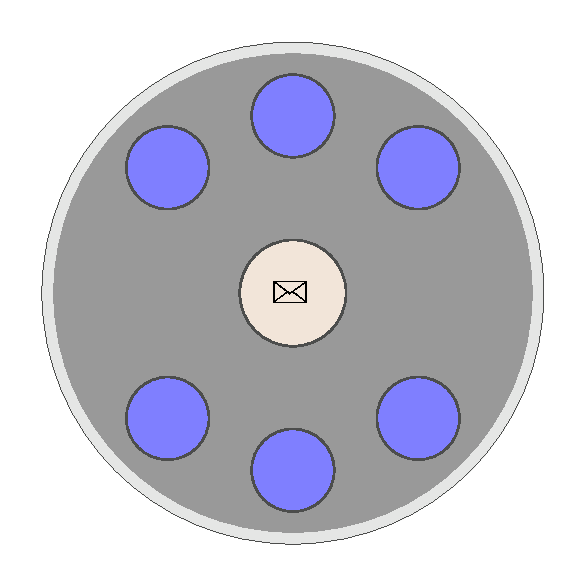
\includegraphics{105_pdfsam_Brief-Kreise-Blau.pdf}};

  \node at (12,0) {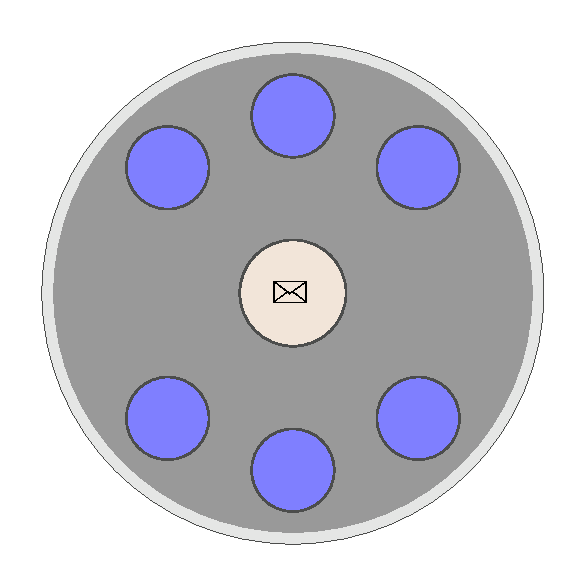
\includegraphics{105_pdfsam_Brief-Kreise-Blau.pdf}};

  \node at (12,12) {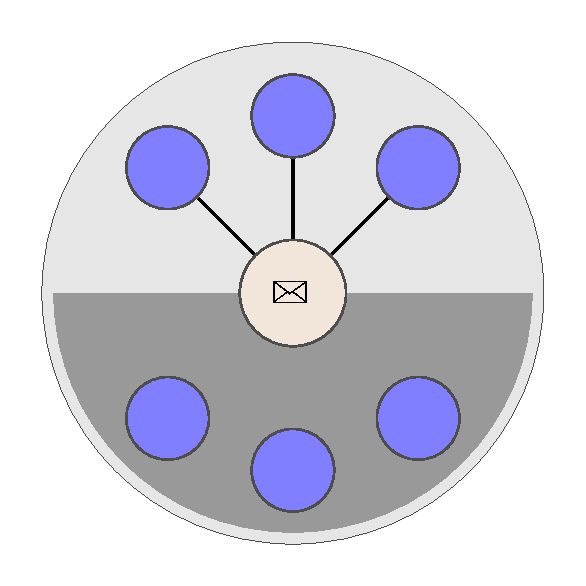
\includegraphics{72_pdfsam_Brief-Kreise-Blau.pdf}};

  \node at (0,12) {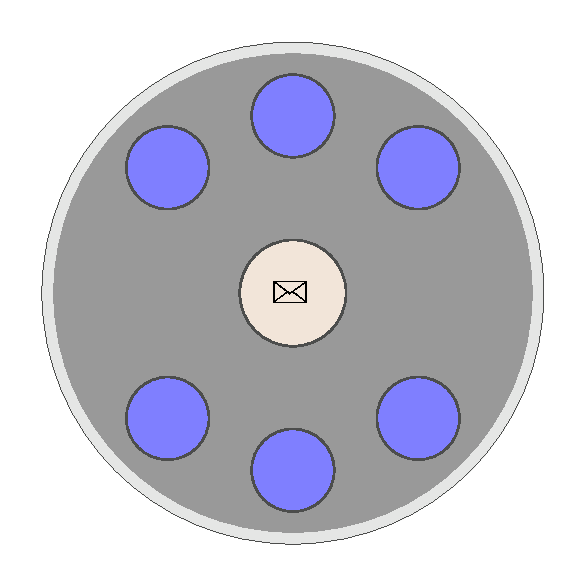
\includegraphics{105_pdfsam_Brief-Kreise-Blau.pdf}};

  \node[draw=black!80,fill=blue!30,ultra thick] at (0,-6)
  {\Huge{Wahr}};

  \node[draw=black!80,fill=blue!30,ultra thick] at (6,-6)
  {\Huge{Falsch}};

  \node[draw=black!80,fill=blue!30,ultra thick] at (12,-6) {\Huge{Mehr Info}};


\end{tikzpicture}

\begin{tikzpicture}[rounded corners]

  \node at (6,18) {\Huge{Genau einer der Briefe ist mit einigen seiner Kreise verbunden.}};

  \node at (0,0) {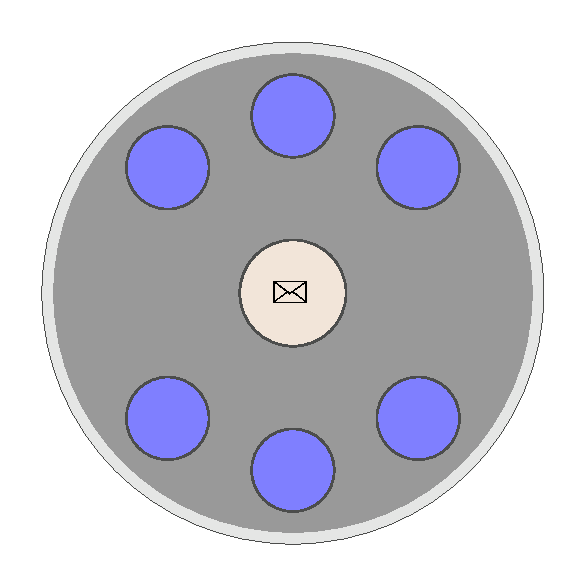
\includegraphics{105_pdfsam_Brief-Kreise-Blau.pdf}};

  \node at (12,0) {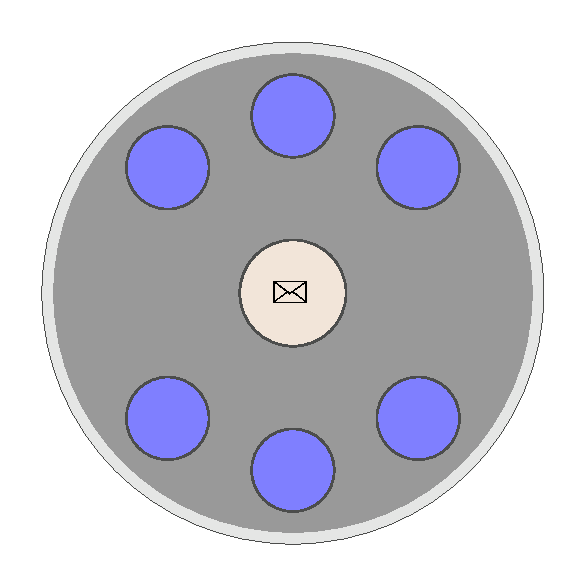
\includegraphics{105_pdfsam_Brief-Kreise-Blau.pdf}};

  \node at (12,12) {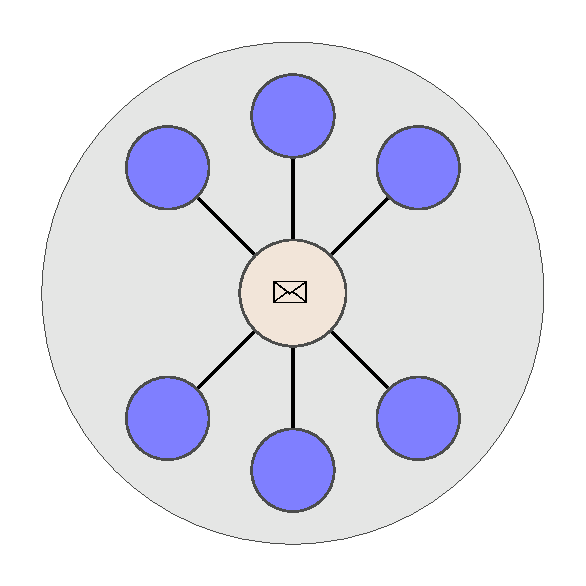
\includegraphics{64_pdfsam_Brief-Kreise-Blau.pdf}};

  \node at (0,12) {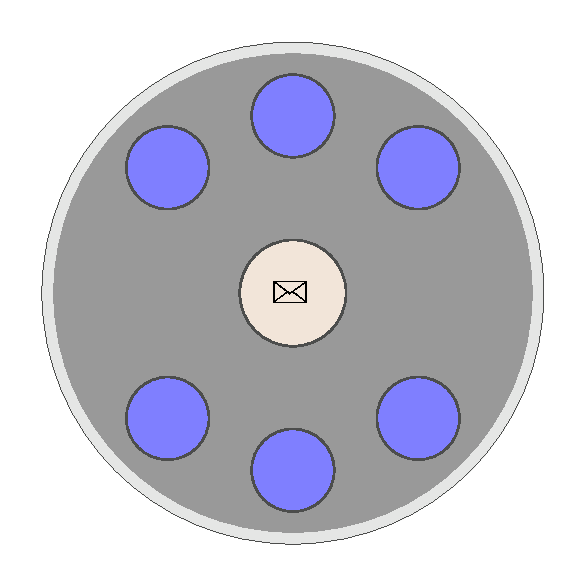
\includegraphics{105_pdfsam_Brief-Kreise-Blau.pdf}};

  \node[draw=black!80,fill=blue!30,ultra thick] at (0,-6)
  {\Huge{Wahr}};

  \node[draw=black!80,fill=blue!30,ultra thick] at (6,-6)
  {\Huge{Falsch}};

  \node[draw=black!80,fill=blue!30,ultra thick] at (12,-6) {\Huge{Mehr Info}};


\end{tikzpicture}

\begin{tikzpicture}[rounded corners]

  \node at (6,18) {\Huge{Genau einer der Briefe ist mit einigen seiner Kreise verbunden.}};

  \node at (0,0) {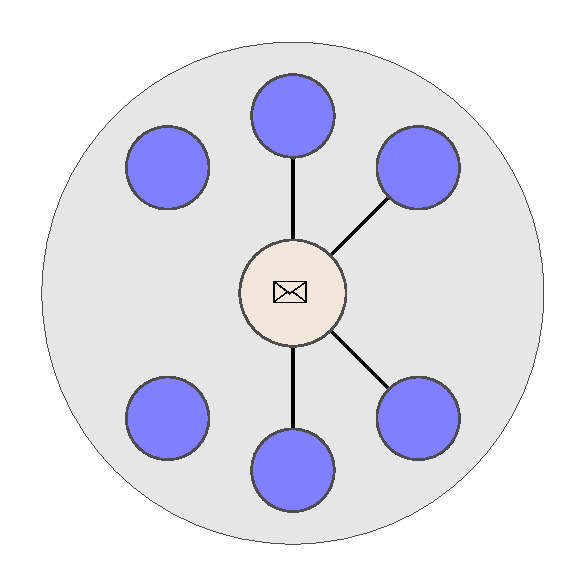
\includegraphics{31_pdfsam_Brief-Kreise-Blau.pdf}};

  \node at (12,0) {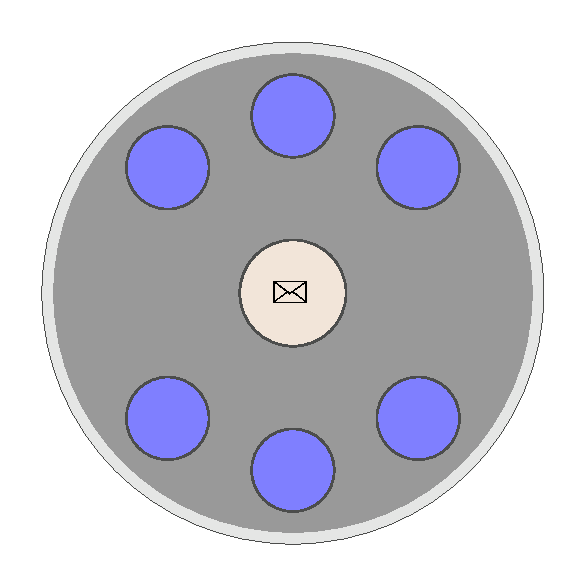
\includegraphics{105_pdfsam_Brief-Kreise-Blau.pdf}};

  \node at (12,12) {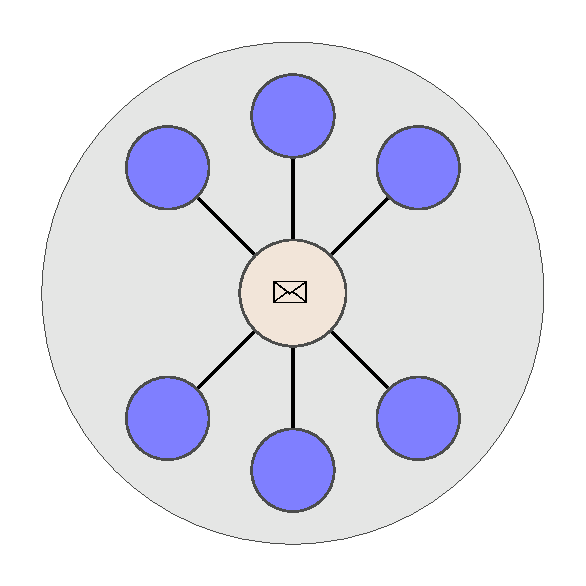
\includegraphics{64_pdfsam_Brief-Kreise-Blau.pdf}};

  \node at (0,12) {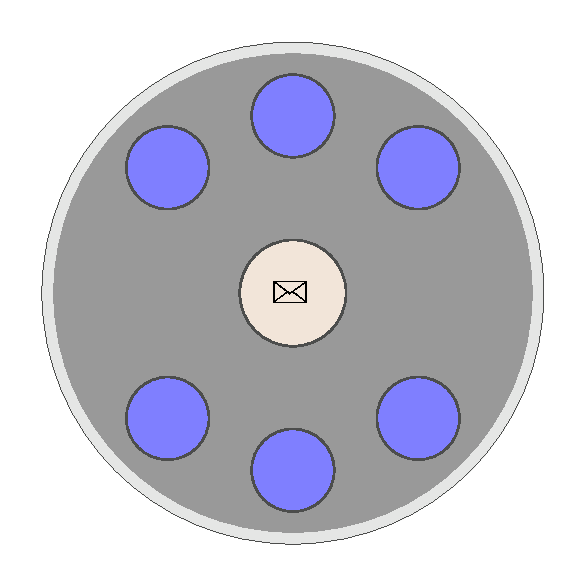
\includegraphics{105_pdfsam_Brief-Kreise-Blau.pdf}};

  \node[draw=black!80,fill=blue!30,ultra thick] at (0,-6)
  {\Huge{Wahr}};

  \node[draw=black!80,fill=blue!30,ultra thick] at (6,-6)
  {\Huge{Falsch}};

  \node[draw=black!80,fill=blue!30,ultra thick] at (12,-6) {\Huge{Mehr Info}};


\end{tikzpicture}


\begin{tikzpicture}[rounded corners]

  \node at (6,18) {\Huge{Genau einer der Briefe ist mit einigen seiner Kreise verbunden.}};

  \node at (0,0) {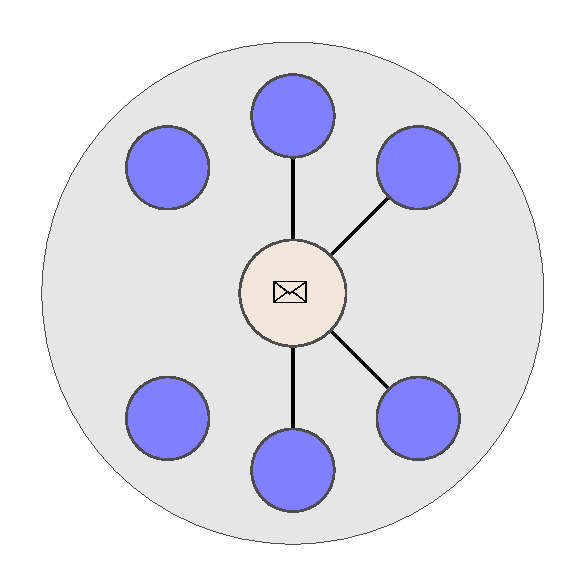
\includegraphics{31_pdfsam_Brief-Kreise-Blau.pdf}};

  \node at (12,0) {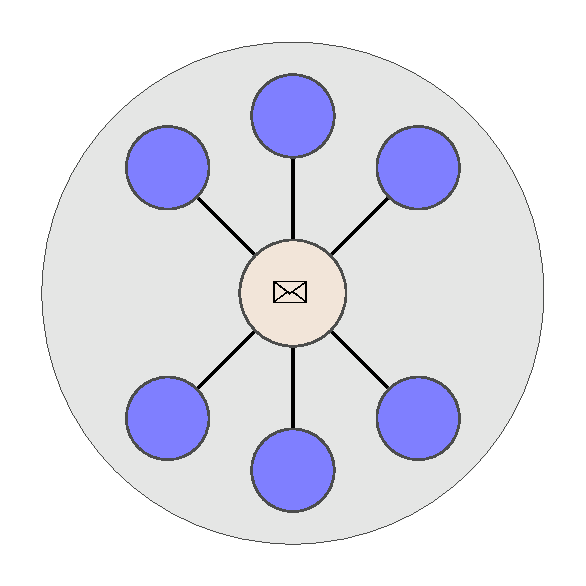
\includegraphics{64_pdfsam_Brief-Kreise-Blau.pdf}};

  \node at (12,12) {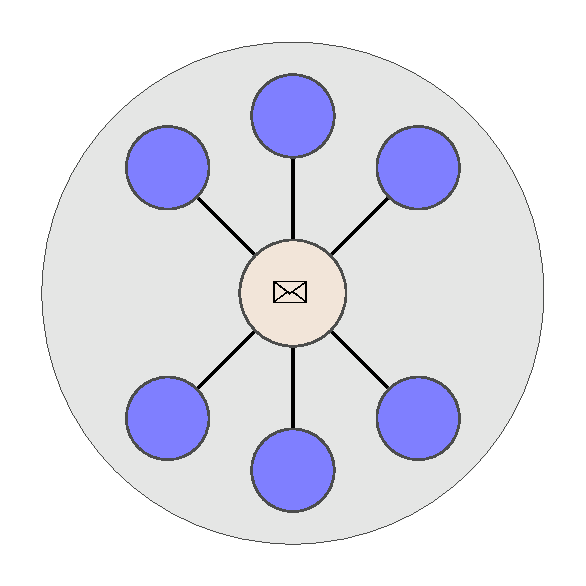
\includegraphics{64_pdfsam_Brief-Kreise-Blau.pdf}};

  \node at (0,12) {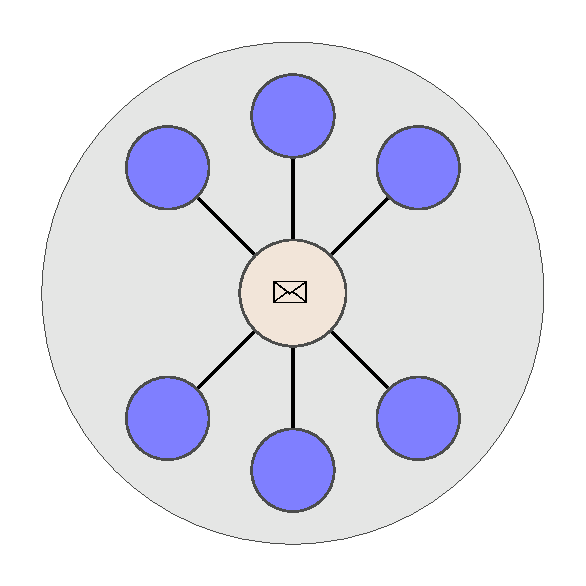
\includegraphics{64_pdfsam_Brief-Kreise-Blau.pdf}};

  \node[draw=black!80,fill=blue!30,ultra thick] at (0,-6)
  {\Huge{Wahr}};

  \node[draw=black!80,fill=blue!30,ultra thick] at (6,-6)
  {\Huge{Falsch}};

  \node[draw=black!80,fill=blue!30,ultra thick] at (12,-6) {\Huge{Mehr Info}};


\end{tikzpicture}


\end{document}

